\chapter{Nguyên lý hoạt động}
\newpage
\fontsize{13}{14}\selectfont
\section{Bộ nguồn}
% Công thức tính toán giá trị và sai số của bộ nguồn.
% giá trị out của hệ thống.
\subsection{Điện áp sau khi chỉnh lưu}

\begin{figure}[H]
	\centering
	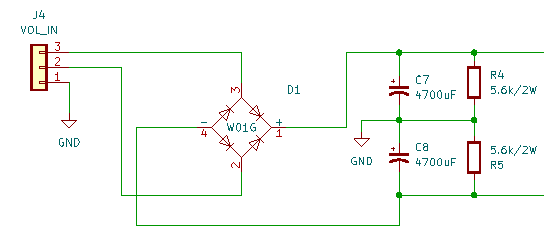
\includegraphics[width=0.6\linewidth]{./picture/mach_chinh_luu.pdf}
	\caption{Mạch chỉnh lưu điện áp đầu vào}
	\label{f_mach chinh luu}
\end{figure}

Giá trị VOL\_IN được cấp bởi đầu ra của biến áp với điện áp đầu ra của biến áp là $12VAC$, sau khi chỉnh lưu toàn sóng với tụ lọc là $C_7$ và $C_8$ thì điện áp ngõ ra của cầu diode được tính toán bằng công thức: \[V_{DC} = \sqrt{2}\times V_{AC} - 2\times V_{diode} \approx 15.6V\]
Trong đó, 
\begin{itemize}[label=-]
	\item $V_{DC}$: là điện áp ngõ ra sau khi chỉnh lưu toán sóng ($V$).
	\item $V_{AC}$: là điện áp ngõ vào cầu diode ($=12V$).
	\item $V_{diode}$: là sụt áp trên hai diode trong cầu chỉnh lưu ($=0.7V$).
\end{itemize}

Tụ $C_{7}$ và $C_{8}$ có chức năng làm giảm độ gợn sóng (ripple) và được tính bằng công thức: \[C = \dfrac{I}{f \times \Delta V} = 5000\mu F \approx 4700\mu F\]
Trong đó,
\begin{itemize}[label = -]
	\item $C$: là giá trị điện dung của tụ ($F$).
	\item $I$: là giá trị dòng tổng ($=1A$).
	\item $f$: là giá trị tần số sau khi chỉnh lưu ($=100Hz$).
	\item $\Delta V$: là độ gợn sóng mong muốn ($=2V$).
\end{itemize}

Điện trở $R_{4}$ và $R_{5}$ được gọi là \textit{Bleeder resistor} có tác dụng xả điện áp ở tụ $C_{7}$ và $C_{8}$ khi ngắt nguồn điện để đảm bảo an toàn cho hệ thống trong những trường hợp nguy hiểm xảy ra gây cho hai tụ này luôn nạp trong thời gian dài. Điện trở này sẽ có giá trị từ $2.2 \sim 10k\Omega$ và công suất từ $2 \sim 10W$.

\subsection{Điện áp cấp $+12V$}

\begin{figure}[H]
	\centering
	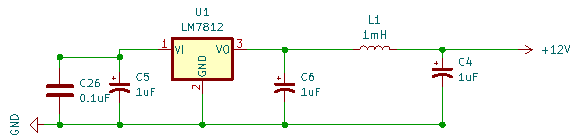
\includegraphics[width=0.6\linewidth]{./picture/supply_+12V.pdf}
	\caption{Mạch cung cấp nguồn $+12V$}
	\label{f_powersupply_+12V}
\end{figure}

Điện áp ngõ vào ($V_{in}$) của mạch cần phải đáp ứng tối thiểu theo công thức: \[ V_{in} > V_{out} + V_{dropout} = 12 + 2 = 14V \rightarrow V_{in} > 14V\]
Trong đó,
\begin{itemize}[label = -]
	\item $V_{in}$: là điện áp đầu vào ($V$).
	\item $V_{out}$: là điện áp đầu ra của LM7812 $=12V$.
	\item $V_{dropout}$: là điện áp rơi trên LM7812 $=2V$.
\end{itemize}

Công suất tiêu tán ($P_{loss}$) là công suất tiêu hao năng lượng dưới dạng nhiệt khi ổn áp: \[ P_{loss} = (V_{in} - V_{out}) \times I_{load} = (15.6 - 12)\times 1 = 3.6W\]
Trong đó,
\begin{itemize}[label=-]
	\item $P_{loss}$: là công suất tiêu tán trên LM7812 ($W$).
	\item $V_{in}$: là điện áp ngõ vào LM7812 ($=15.6V$).
	\item $V_{out}$: là điện áp ngõ ra LM7812 ($=12$).
	\item $I_{load}$: là dòng tải ($=1A$).
\end{itemize}

Kích thước tản nhiệt ($R_{th}$) để đảm bảo IC không quá nóng, nhiệt độ $T_j$ phải nằm trong giới hạn ($T_j \leq 125^{\circ}C$). Ta sử dụng công thức: \[ T_{j} = T_{o} + P_{loss} \times R_{th(tot)} \rightarrow R_{th(tot)} \leq \dfrac{T_{j} - T_{o}}{P_{loss}} = \dfrac{125 - 25}{3.6} \approx 27.8 \rightarrow R_{th(tot)} \leq 27.8^{\circ}C/W
 \]
 \[ \Rightarrow R_{th(c-a)} \leq R_{th(tot)} - R_{th(j-c)} = 27.8 - 5 \rightarrow R_{th(c-a)} \leq 22.8^{\circ}C/W \]
Trong đó,
\begin{itemize}[label = -]
	\item $T_{j}$: là nhiệt độ cho phép hoạt động của IC ($ ^\circ C$).
	\item $T_{o}$: là nhiệt độ của môi trường ($=25^{\circ}C$).
	\item $P_{loss}$: là công suất tiêu tán trên LM7812 ($=3.6W$).
	\item $R_{th(tot)}$: là tổng trở nhiệt từ junction đến môi trường ($27.8^{\circ}C/W$).
	\item $R_{th(j-c)}$: là trở nhiệt junction-to-case ($=5^{\circ}C/W$).
	\item $R_{th(c-a)}$: là trở nhiệt case-to-air ($^{\circ}C/W$).
\end{itemize}

Tụ điện đầu vào $C_{5}$ giúp bù sụt áp tạm thời và có giá trị là $1\mu F$.

Tụ điện đầu ra $C_{4}$ và $C_6$ giúp cải thiện ổn định điện áp đầu ra và có giá trị là $1\mu F$.

Tụ $C_{26}$ là tụ điện có chức năng dập nhiễu cao tần có giá trị là $0.1\mu F$.

Cuộn cảm $L_{1}$ có chức năng loại bỏ các nhiễu tần số cao có thể xuất hiện đầu ra, và tạo thành một bộ lọc LC giúp làm mịn điện áp đầu ra bằng cách giảm biên độ của các gợn sóng còn lại sau khi chỉnh lưu và ổn áp.

Hiệu suất ($\eta$) của mạch được tính bằng công thức: \[ \eta = \dfrac{V_{out}\times I_{load}}{V_{in} \times I_{load}}\times 100\% = \dfrac{12\times 1}{15.6 \times 1}\times 100\% \approx 76.9\% \]

\subsection{Điện áp cấp $-12V$}

\begin{figure}[H]
	\centering
	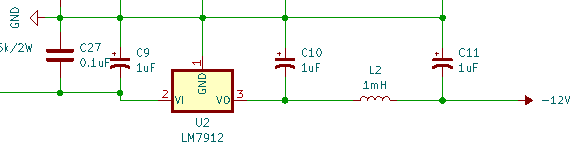
\includegraphics[width=0.6\linewidth]{./picture/supply_-12V.pdf}
	\caption{Mạch cung cấp nguồn $-12V$}
	\label{f_powersupply_-12V}
\end{figure}

Điện áp ngõ vào ($V_{in}$) của mạch cần phải đáp ứng tối thiểu theo công thức: \[ V_{in} < V_{out} - V_{dropout} = -12 - 2 = -14V \rightarrow V_{in} < -14V\]
Trong đó,
\begin{itemize}[label = -]
	\item $V_{in}$: là điện áp đầu vào ($V$).
	\item $V_{out}$: là điện áp đầu ra của LM7912 $=-12V$.
	\item $V_{dropout}$: là điện áp rơi trên LM7912 $=2V$.
\end{itemize}

Công suất tiêu tán ($P_{loss}$) là công suất tiêu hao năng lượng dưới dạng nhiệt khi ổn áp: \[ P_{loss} = (|V_{in}| - |V_{out}|) \times I_{load} = (15.6 - 12)\times 1 = 3.6W\]
Trong đó,
\begin{itemize}[label=-]
	\item $P_{loss}$: là công suất tiêu tán trên LM7912 ($W$).
	\item $V_{in}$: là điện áp ngõ vào LM7812 ($=-15.6V$).
	\item $V_{out}$: là điện áp ngõ ra LM7812 ($=-12$).
	\item $I_{load}$: là dòng tải ($=1A$).
\end{itemize}

Kích thước tản nhiệt ($R_{th}$) để đảm bảo IC không quá nóng, nhiệt độ $T_j$ phải nằm trong giới hạn ($T_j \leq 125^{\circ}C$). Ta sử dụng công thức: \[ T_{j} = T_{o} + P_{loss} \times R_{th(tot)} \rightarrow R_{th(tot)} \leq \dfrac{T_{j} - T_{o}}{P_{loss}} = \dfrac{125 - 25}{3.6} \approx 27.8 \rightarrow R_{th(tot)} \leq 27.8^{\circ}C/W
\]
\[ \Rightarrow R_{th(c-a)} \leq R_{th(tot)} - R_{th(j-c)} = 27.8 - 5 \rightarrow R_{th(c-a)} \leq 22.8^{\circ}C/W \]
Trong đó,
\begin{itemize}[label = -]
	\item $T_{j}$: là nhiệt độ cho phép hoạt động của IC ($ ^\circ C$).
	\item $T_{o}$: là nhiệt độ của môi trường ($=25^{\circ}C$).
	\item $P_{loss}$: là công suất tiêu tán trên LM7912 ($=3.6W$).
	\item $R_{th(tot)}$: là tổng trở nhiệt từ junction đến môi trường ($27.8^{\circ}C/W$).
	\item $R_{th(j-c)}$: là trở nhiệt junction-to-case ($=5^{\circ}C/W$).
	\item $R_{th(c-a)}$: là trở nhiệt case-to-air ($^{\circ}C/W$).
\end{itemize}

Tụ điện đầu vào $C_{9}$ giúp bù sụt áp tạm thời và có giá trị là $1\mu F$.

Tụ điện đầu ra $C_{10}$ và $C_{11}$ giúp cải thiện ổn định điện áp đầu ra và có giá trị là $1\mu F$.

Tụ $C_{27}$ là tụ điện có chức năng dập nhiễu cao tần có giá trị là $0.1\mu F$.

Cuộn cảm $L_{2}$ có chức năng loại bỏ các nhiễu tần số cao có thể xuất hiện đầu ra, và tạo thành một bộ lọc LC giúp làm mịn điện áp đầu ra bằng cách giảm biên độ của các gợn sóng còn lại sau khi chỉnh lưu và ổn áp.

Hiệu suất ($\eta$) của mạch được tính bằng công thức: \[ \eta = \dfrac{V_{out}\times I_{load}}{V_{in} \times I_{load}}\times 100\% = \dfrac{12\times 1}{15.6 \times 1}\times 100\% \approx 76.9\% \]

\subsection{Điện áp cấp $+5V$}

\begin{figure}[H]
	\centering
	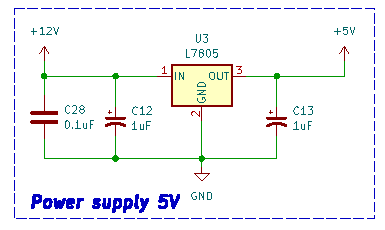
\includegraphics[width=0.6\linewidth]{./picture/power_supply_5V.pdf}
	\caption{Mạch cung cấp nguồn $+5V$}
	\label{f_supply_+5V}
\end{figure}

Điện áp ngõ vào ($V_{in}$) của mạch cần phải đáp ứng tối thiểu theo công thức: \[ V_{in} > V_{out} + V_{dropout} = 5 + 2 = 7V \rightarrow V_{in} > 7V\]
Trong đó,
\begin{itemize}[label = -]
	\item $V_{in}$: là điện áp đầu vào ($V$).
	\item $V_{out}$: là điện áp đầu ra của LM7805 $=5V$.
	\item $V_{dropout}$: là điện áp rơi trên LM7805 $=2V$.
\end{itemize}

Công suất tiêu tán ($P_{loss}$) là công suất tiêu hao năng lượng dưới dạng nhiệt khi ổn áp: \[ P_{loss} = (V_{in} - V_{out}) \times I_{load} = (12 - 5)\times 1 = 7W\]
Trong đó,
\begin{itemize}[label=-]
	\item $P_{loss}$: là công suất tiêu tán trên LM7805 ($W$).
	\item $V_{in}$: là điện áp ngõ vào LM7805 ($=12V$).
	\item $V_{out}$: là điện áp ngõ ra LM7805 ($=5V$).
	\item $I_{load}$: là dòng tải ($=1A$).
\end{itemize}

Kích thước tản nhiệt ($R_{th}$) để đảm bảo IC không quá nóng, nhiệt độ $T_j$ phải nằm trong giới hạn ($T_j \leq 125^{\circ}C$). Ta sử dụng công thức: \[ T_{j} = T_{o} + P_{loss} \times R_{th(tot)} \rightarrow R_{th(tot)} \leq \dfrac{T_{j} - T_{o}}{P_{loss}} = \dfrac{125 - 25}{7} \approx 14.3 \rightarrow R_{th(tot)} \leq 14.3^{\circ}C/W
\]
\[ \Rightarrow R_{th(c-a)} \leq R_{th(tot)} - R_{th(j-c)} = 14.3 - 5 \rightarrow R_{th(c-a)} \leq 9.3^{\circ}C/W \]
Trong đó,
\begin{itemize}[label = -]
	\item $T_{j}$: là nhiệt độ cho phép hoạt động của IC ($ ^\circ C$).
	\item $T_{o}$: là nhiệt độ của môi trường ($=25^{\circ}C$).
	\item $P_{loss}$: là công suất tiêu tán trên LM7805 ($=7W$).
	\item $R_{th(tot)}$: là tổng trở nhiệt từ junction đến môi trường ($14.3^{\circ}C/W$).
	\item $R_{th(j-c)}$: là trở nhiệt junction-to-case ($=5^{\circ}C/W$).
	\item $R_{th(c-a)}$: là trở nhiệt case-to-air ($^{\circ}C/W$).
\end{itemize}

Tụ điện đầu vào $C_{12}$ giúp bù sụt áp tạm thời và có giá trị là $1\mu F$.

Tụ điện đầu ra $C_{13}$ giúp cải thiện ổn định điện áp đầu ra và có giá trị là $1\mu F$.

Tụ $C_{28}$ là tụ điện có chức năng dập nhiễu cao tần có giá trị là $0.1\mu F$.

Hiệu suất ($\eta$) của mạch được tính bằng công thức: \[ \eta = \dfrac{V_{out}\times I_{load}}{V_{in} \times I_{load}}\times 100\% = \dfrac{5\times 1}{12 \times 1}\times 100\% \approx 41.7\% \]

\subsection{Điện áp cấp $+3.3V$}

\begin{figure}[H]
	\centering
	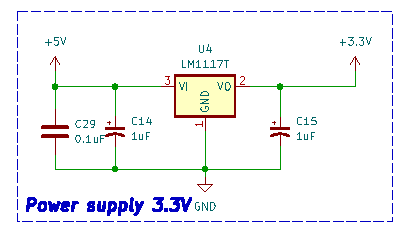
\includegraphics[width=0.6\linewidth]{./picture/power_supply_3V.pdf}
	\caption{Mạch cung cấp nguồn $+3.3V$}
	\label{f_supply_+3.3V}
\end{figure}

Điện áp ngõ vào ($V_{in}$) của mạch cần phải đáp ứng tối thiểu theo công thức: \[ V_{in} > V_{out} + V_{dropout} = 3.3 + 1.2 = 4.5V \rightarrow V_{in} > 4.5V\]
Trong đó,
\begin{itemize}[label = -]
	\item $V_{in}$: là điện áp đầu vào ($V$).
	\item $V_{out}$: là điện áp đầu ra của LM7805 $=3.3V$.
	\item $V_{dropout}$: là điện áp rơi trên LM7805 $=1.2V$.
\end{itemize}

Công suất tiêu tán ($P_{loss}$) là công suất tiêu hao năng lượng dưới dạng nhiệt khi ổn áp: \[ P_{loss} = (V_{in} - V_{out}) \times I_{load} = (5 - 3.3)\times 1 = 1.7W\]
Trong đó,
\begin{itemize}[label=-]
	\item $P_{loss}$: là công suất tiêu tán trên LM117T ($W$).
	\item $V_{in}$: là điện áp ngõ vào LM117T ($=5V$).
	\item $V_{out}$: là điện áp ngõ ra LM117T ($=3.3$).
	\item $I_{load}$: là dòng tải ($=1A$).
\end{itemize}

Kích thước tản nhiệt ($R_{th}$) để đảm bảo IC không quá nóng, nhiệt độ $T_j$ phải nằm trong giới hạn ($T_j \leq 125^{\circ}C$). Ta sử dụng công thức: \[ T_{j} = T_{o} + P_{loss} \times R_{th(tot)} \rightarrow R_{th(tot)} \leq \dfrac{T_{j} - T_{o}}{P_{loss}} = \dfrac{125 - 25}{1.7} \approx 58.8 \rightarrow R_{th(tot)} \leq 58.8^{\circ}C/W
\]
\[ \Rightarrow R_{th(c-a)} \leq R_{th(tot)} - R_{th(j-c)} = 58.8 - 2 \rightarrow R_{th(c-a)} \leq 56.8^{\circ}C/W \]
Trong đó,
\begin{itemize}[label = -]
	\item $T_{j}$: là nhiệt độ cho phép hoạt động của IC ($ ^\circ C$).
	\item $T_{o}$: là nhiệt độ của môi trường ($=25^{\circ}C$).
	\item $P_{loss}$: là công suất tiêu tán trên LM117T ($=7W$).
	\item $R_{th(tot)}$: là tổng trở nhiệt từ junction đến môi trường ($58.8^{\circ}C/W$).
	\item $R_{th(j-c)}$: là trở nhiệt junction-to-case ($=2^{\circ}C/W$).
	\item $R_{th(c-a)}$: là trở nhiệt case-to-air ($^{\circ}C/W$).
\end{itemize}

Tụ điện đầu vào $C_{14}$ giúp bù sụt áp tạm thời và có giá trị là $1\mu F$.

Tụ điện đầu ra $C_{15}$ giúp cải thiện ổn định điện áp đầu ra và có giá trị là $1\mu F$.

Tụ $C_{29}$ là tụ điện có chức năng dập nhiễu cao tần có giá trị là $0.1\mu F$.

Hiệu suất ($\eta$) của mạch được tính bằng công thức: \[ \eta = \dfrac{V_{out}\times I_{load}}{V_{in} \times I_{load}}\times 100\% = \dfrac{3.3\times 1}{5 \times 1}\times 100\% = 66\% \]

\section{Bộ tiền lọc của hệ thống}
% Thực hiện nêu ra các công thức tính toán cho bộ tiền lọc
% cho chế độ DC thì nêu công thức tính các điện trở và sai số đầu ra so với tín hiệu đầu vào
% cho chế độ AC thì nêu công thức tính các điện trở, cách dời offset và sai số giữa đầu ra so với tín hiệu đầu vào
\subsection{Bộ tiền lọc của chế độ đo DC}

\begin{figure}[H]
	\centering
	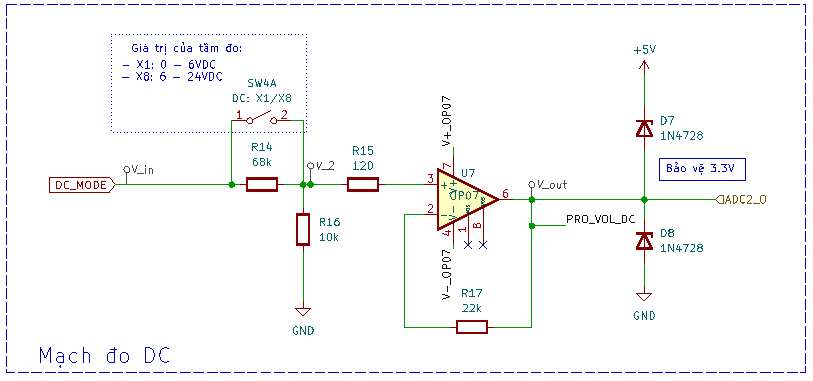
\includegraphics[width=0.6\linewidth]{./picture/board_DC.pdf}
	\caption{Mạch tiền lọc đo điện áp DC}
	\label{f_board_Dc}
\end{figure}

\begin{itemize}[label = -]
	\item Ở chế độ (X1): 
		\begin{itemize}[label = +]
			\item $V_2$: $V_2 = V_in$.
			\item $A_{v}$: $ A_{v} = 1 + \dfrac{R_{17}}{R_{in}} = 1 + \dfrac{22K}{50M} \approx 1$.
			\item $\Delta V$: $\Delta V = 60 \mu s$.
			\item $\%\sigma_{V}$: $\%\sigma_{V} = \dfrac{\Delta V}{V_{in_{max}}}\times 100\% = \dfrac{60\mu }{3} = 0.002\%$.
		\end{itemize}
	\item Ở chế độ (X8):
		\begin{itemize}[label = +]
			\item $V_2$: $V_2 =  V_{in} \times \dfrac{R16}{R14 + R16} = V_{in} \times \dfrac{10K}{10K + 68K}$.
			\item $A_{v}$: $ A_{v} = 1 + \dfrac{R_{17}}{R_{in}} = 1 + \dfrac{22K}{50M} \approx 1$.
			\item $\Delta V$: $\Delta V = \Delta V + \Delta V_2 = 60\mu V + V_{in} \times\dfrac{10K\times 1\%}{10K\times 1\% + 68K\times 1\%} = 60 + V_{in} \times 128205.1282 (\mu V)$.
			\item $\%\sigma_{V}$: $\%\sigma_{V} = \dfrac{\Delta V}{V_{in_{max}}}\times 100\% = \dfrac{60\mu + 24\times128205.1282\mu}{24} \approx 12.82\%$.
		\end{itemize}
\end{itemize}

\subsection{Bộ tiền lọc của chế độ đo AC}

\begin{figure}[H]
	\centering
	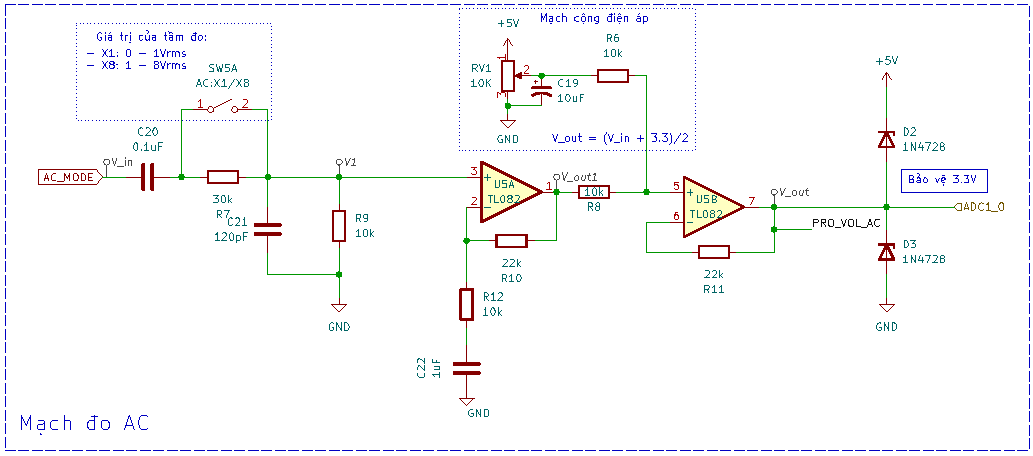
\includegraphics[width=0.6\linewidth]{./picture/board_AC.pdf}
	\caption{Mạch tiền lọc đo điện áp AC}
	\label{f_board_Ac}
\end{figure}

\begin{itemize}[label = -]
	\item Ở chế độ (X1):
		\begin{itemize}[label = +]
			\item $V_1$: $V_{1} = V_{in}$.
			\item $A_{v}$: $A_{v} \approx 1$.
			\item $\Delta V$: $\Delta V = \Delta V + \Delta V_{5} = 3mV + \Delta V_{5}$.
			\item $\%\sigma_{V}$: $\%\sigma_{V} = \dfrac{\Delta V}{V_{in_{max}}} \times 100\% = \dfrac{3m + 0.5}{3} \times 100\% = 16.77\%$
		\end{itemize}
	\item Ở chế độ (X8):
		\begin{itemize}[label = +]
			\item $V_1$: $V_{1} = V_{in} \times \dfrac{R9}{R7 + R9} = V_{in}\times \dfrac{10K}{30K + 10K}$.
			\item $A_{v}$: $A_{v} \approx 1$.
			\item $\Delta V$: $\Delta V = \Delta V + \Delta V_{5} + \Delta V_{1}= 3mV + \Delta V_{5} + \dfrac{10K \times 1\%}{10K\times 1\% + 30K\times 1\%}\times V_{in} = 3m + \Delta V_{5} + 0.25\times V_{in}$.
			\item $\%\sigma_{V}$: $\%\sigma_{V} = \dfrac{\Delta V}{V_{in_{max}}} \times 100\% = \dfrac{3m + 0.5 + 0.25\times22}{22} \times 100\% = 27.29\%$
		\end{itemize}
\end{itemize}

\section{Chuyển đổi điện áp}
% Thực hiện nêu ra lý thuyết của ADC số bit, tầm đo, sai số của ADC
% thời gian chuyển đổi của bộ ADC và tốc độ đáp ứng của bộ ADC
\subsection{Chế độ ADC}

\begin{figure}[H]
	\centering
	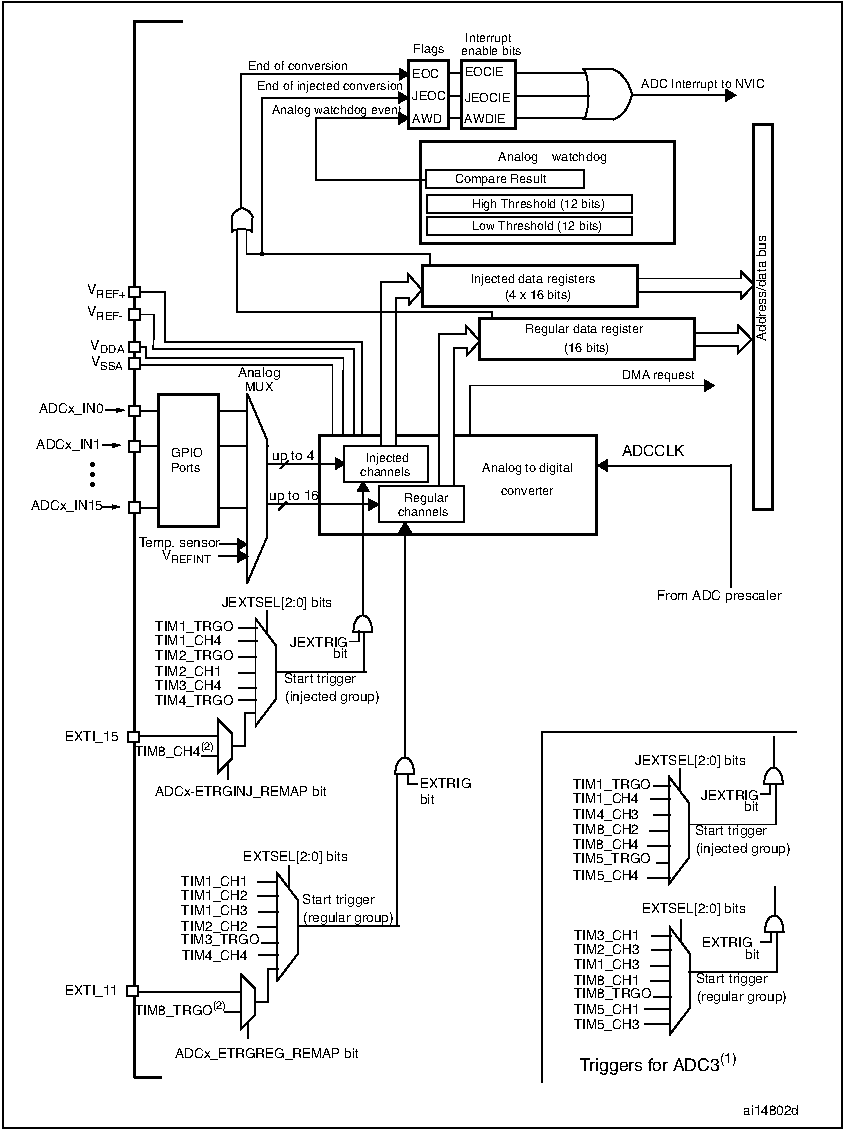
\includegraphics[width=0.7\linewidth]{./picture/Single ADC block diagram.pdf}
	\caption{Sơ đồ khối của bộ ADC của STM32F1xx}
	\label{f_single adc block diagram}
\end{figure}



\subsubsection{Bước lượng tử hóa của bộ ADC}

Với bộ ADC của STM32F1xx thì ta sử dụng chế độ chuyển đổi liên tục với điện áp $V_{ref+} = 3.3V$ và $V_{ref-} = 0V$, số bit lượng tử là $B= 12$ bit. Suy ra bước lượng tử hóa của bộ ADC là: \[ Q = \dfrac{R}{2^{B}} = \dfrac{3.3}{2^{12}} \approx 0.88057mV \]

\subsubsection{Sai số hiệu dụng $e_{rms}$}

Sai số hiệu dụng $e_{rms}$ là chỉ số quan trọng đánh giá độ chính xác, biểu thị mức độ nhiễu và sai số tổng hợp trong quá trình chuyển đổi tín hiệu, được tính bởi công thức: \[ e_{rms} = \sigma_{q} = \sqrt{\bar{e}^{2}} = \dfrac{Q}{\sqrt{12}} = \dfrac{0.88057mV}{\sqrt{12}} \approx 254.1987 \mu V \]

\subsubsection{Sai số của bộ ADC}

Sai số của bộ ADC thường được chịu ảnh hưởng bởi một số yếu tố, bao gồm độ phân giải, nhiễu, đặc điểm của nguồn tham chiếu, và đặc tính phần của cứng của STM32F1xx.

\begin{itemize}[label=-]
	\item Độ phân giải ADC: bộ ADC của STM32F1xx có số bit lượng tử là 12-bit, suy ra sai số lý thuyết là: $\pm \dfrac{1}{2}\times Q = \pm\dfrac{1}{2}\times 0.88057mV \approx \pm440.285\mu V$ .
	\item Sai số tổng thể của ADC:\\
		\begin{enumerate}[label = \alph*)]
			\item Total Unadjusted Error (TUE): là sai số của tất cả nguồn sai số, chẳng hạn như sai số tuyến tính, sai số bù, và nhiễu. TUE được tính bằng công thức: \[TUE = \sqrt{(OffsetError)^{2} + (GainError)^{2} + (LinearError)^{2} + (NoiseError)^{2}}\]
			và thường được cho một giá trị dao động từ $\pm 1Q \sim \pm 4Q \Leftrightarrow \pm0.88057 \sim \pm 3.52228 (mV)$.
			\item Differential Non-Linearity (DNL): là đo độ không tuyến tính giữa các bước ADC liên tiếp. Nếu DNL $>\pm 1Q$, ADC sẽ có thể mất tính đơn điệu. DNL được tính bằng công thức: \[DNL = \dfrac{V_{out}(i + 1) - V_{out}(i)}{Q} - 1\]
			Nếu:\\
				\begin{itemize}[label = +]
					\item DNL = 0: độ tuyến tính hoàn hoản, mỗi bước ADC đều có độ rộng bằng nhau.
					\item DNL > 0: bước ADC lớn hơn bước lý tưởng.
					\item DNL < 0: bước ADC nhỏ hơn bước lý tưởng.
					\item DNL > $1Q$: có thể gây ra mất tính đơn điệu, dẫn đến các mã bị thiếu.
				\end{itemize}
			Giá trị DNL thường nằm trong khoảng $\pm 0.5Q \sim \pm Q \Leftrightarrow \pm 0.44029 \sim \pm 0.88057 (mV)$.
			\item Integral Non-Linearity (INL): là đo độ lệch của đặc tuyến thực tế của ADC so với đường lý tưởng. INL càng nhỏ, độ chính xác càng cao, và được tính bằng công thức: \[INL(i) = \dfrac{V_{out}(i) - V_{ideal}(i)}{Q}\]
			Nếu:\\
				\begin{itemize}[label = +]
					\item INL = 0: độ tuyến tính hoàn hảo, đặc tuyến thực tế trùng với được lý tưởng.
					\item INL > 0: đặc tuyến thực tế nằm trên đường lý tưởng.
					\item INL < 0: đặc tuyến thực tế nằm dưới đường lý tưởng.
				\end{itemize}
			\item Offset Error: là độ lệch đầu ra ADC so với giá trị lý thuyết ở đầu vào bằng 0V. Và giá trị này thường nằm trong khoảng $\pm 1Q \sim \pm 2Q \Leftrightarrow \pm 0.88057 \sim \pm 1.76114 (mV)$.
			\item Gain Error: là sai số do độ dốc của đường đặc tuyến chuyển đổi không đúng, được tính bởi công thức: \[Gain Error = \left( \dfrac{V_{out} - V_{ideal}}{V_{ideal}} \right) \times 100\%\] và thường nằm trong khoảng $\pm 0.5\% \sim \pm 1\%$.
			\item Sai số ở nguồn tham chiếu ($V_{ref}$): là sai số gây ra sử dụng điện áp tham chiếu có sai số gây ảnh hưởng đến độ chính xác sau chuyển đổi.
			\item Sai số do tốc độ lấy mẫu (sampling timer): thời gian lấy mẫu quá ngắn có thể dẫn đến lỗi lấy mẫu (sampling error).
		\end{enumerate}
\end{itemize}

\subsubsection{Thời gian hoàn thành việc chuyển đổi tín hiệu}

Bộ ADC được thiết lập với tần số hoạt động $f_{ADC} = 36MHz \rightarrow t_{ADC} \approx 27.7778 ns$. Thời gian hoàn thành việc chuyển đổi tín hiệu từ tín hiệu analog sang tín hiệu digital được tính bởi công thức: \[T_{final} = T_{sampling} + T_{conv}\] trong đó,

\begin{itemize}[label= -]
	\item $T_{final}$: là thời gian hoàn thành việc chuyển đổi ($s$).
	\item $T_{sampling}$: là thời gian lấy mẫu $T_{sampling} = N_{cycles sampline} \times t_{ADC}$.
	\item $T_{conv}$: là thời gian chuyển đổi lõi $T_{conv} = N_{cycles conversion} \times t_{ADC}$.
\end{itemize}

\[\Leftrightarrow T_{final} = (N_{cycles sampline} + N_{cycles conversion}) \times t_{ADC}\]

	\begin{enumerate}[label = \alph *)]
		\item Tốc độ lấy mẫu của PA1 (chế độ đo AC): với $N_{cycles sampline} = 1.5 cycle$ và $N_{cycles conversion} = 41.5 cycle$, vậy thời gian chuyển đổi xong của bộ ADC ở chế độ AC là: \[T_{finalAC} = (1.5 + 41.5) \times 27.7778ns \approx 1.1944 \mu s\]
		\[\Rightarrow f_{AC} = \dfrac{1}{T_{finalAC}} \approx 837.24KHz\]
		\item Tốc độ lấy mẫu của PA2 (chế độ đo DC): với $N_{cycles sampline} = 1.5 cycle$ và $N_{cycles conversion} = 239.5 cycle$, vậy thời gian chuyển đổi xong của bộ ADC ở chế độ DC là: \[T_{finalDC} = (1.5 + 239.5) \times 27.7778ns \approx 6.6944 \mu s\]
		\[\Rightarrow f_{DC} = \dfrac{1}{T_{finalDC}} \approx = 149.377KHz\]
	\end{enumerate}

\subsection{Chế độ DMA}

\begin{figure}[H]
	\centering
	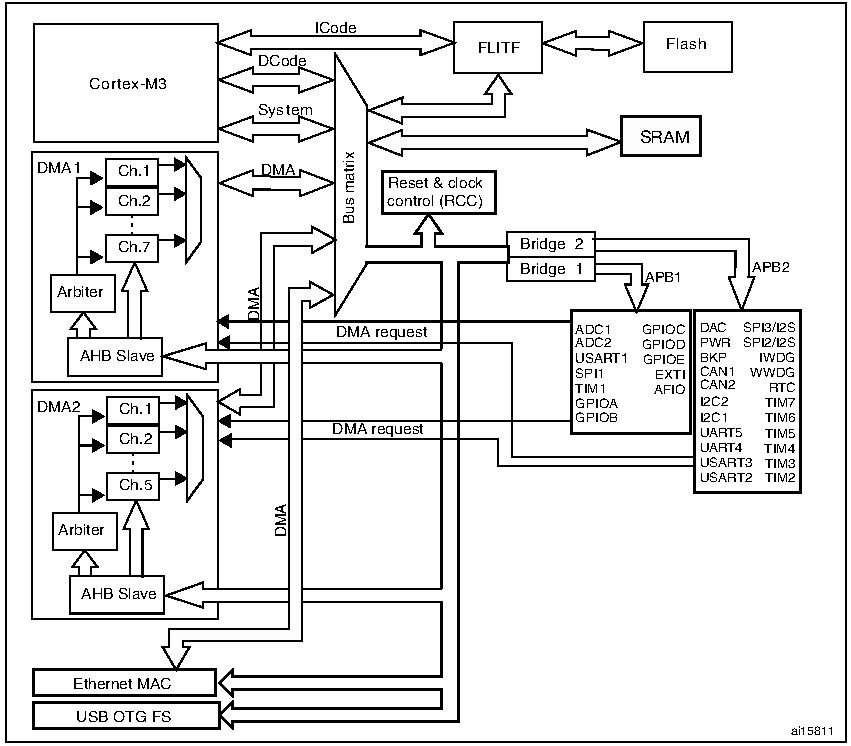
\includegraphics[width=0.7\linewidth]{./picture/DMA block diagram in connectivity line devices.pdf}
	\caption{Sơ đồ khối của bộ DMA của STM32F10xx}
	\label{f_DMA block diagram in connectivity line devices}
\end{figure}

Sử dụng chế độ DMA để tiến hành lưu trữ dữ liệu khi được được từ ADC trả về và lưu vào một buffer để chứa giá trị đó. DMA hoạt động ở hai chế độ:

\begin{itemize}[label = -]
	\item Normal Mode: DMA dừng hoạt động sau khi truyền đủ số lượng dữ liệu xác định bởi NDTR. Bạn cần khởi động lại DMA thủ công.
	\item Circular Mode: DMA liên tục ghi đè giá trị ADC vào buffer khi buffer đầy. Điều này hữu ích cho các ứng dụng yêu cầu lưu trữ liên tục (như xử lý tín hiệu thời gian thực).
\end{itemize}

Với STM32F10xx thì có 64Kbyte static SRAM, và có thể truy cập được dưới dạng Byte, Half-words (16-bit) và Words (32-bit). Địa chỉ của SRAM bắt đầu từ 0x2000 0000. Trong đó thì pham vi của địa chỉ của DMA trong SRAM là:

\begin{table}[H]
	\centering
	\begin{tabular}{|c|c|c|}
		\hline
		Boundary address & Peripheral & Bus \\
		\hline
		0x4002 0000 - 0x4002 03FF & DMA1 & \multirow{2}{*}{AHB} \\
		\cline{1 - 2}
		0x4002 0400 - 0x4002 07FF & DMA2 & \\
		\hline
	\end{tabular}
	\caption{Bảng địa chỉ của DMA trong SRAM}
	\label{t_address DMA in SRAM}
\end{table}



\begin{lstlisting}
	#define ADC_BUFFER_SIZE 1000
	
	uint16_t OSC_Buf[ADC_BUFFER_SIZE];
	HAL_ADC_Start_DMA(&hadc1, (uint32_t *)OSC_Buf, sizeof(OSC_Buf));
\end{lstlisting}

Với giá trị $\texttt{ADC\_BUFFER\_SIZE} = 1000$ và bộ ADC lấy mẫu ở chế độ AC là $t_{finalAC} \approx 1.1944 \mu s$, thì giá trị mà để đưa con trỏ về lại vị trí ban đầu trong buffer là: \[ t_{buf} = t_{finalAC} \times ADC\_BUFFER\_SIZE = 1.1944\mu s \times 1000 = 1.1944ms \]

Như vậy, cần tối thiểu là $1.1944ms$ để bộ DMA lưu trữ hết giá trị của buffer.

\section{Tính toán giá trị và hiển thị giá trị}
% Chủ yếu liên quan đến các hàm xử lý trong timer và công thức tính toán liên quan đến việc tính toán các giá trị hiển thị lên LCD
% tính sai số của biến hiển thị lên LCD từ HEX
\subsection{Tính toán giá trị ở chế độ AC}

Giá trị chuyển đổi giá trị thực tế từ bộ ADC được thực hiện bởi hàm:
\begin{lstlisting}
	/**
	* @brief  Calculate AC voltage from ADC value.
	* @param  HEX: ADC raw value (0-4095 for 12-bit ADC).
	* @param  Range: Measurement range (scaling factor).
	* @retval Calculated AC voltage.
	*/
	float ValueVac(uint32_t HEX, uint16_t Range) {
		float Temp = 0.0;
		Temp = (float)(((2 * (HEX * 3.3) / 4096.0) - 3.3) * Range);
		return Temp;
	}
	
\end{lstlisting}
 Trong chế độ AC, ta cần phải tính toán 2 giá trị là:
 
\begin{itemize}[label = -]
	\item \texttt{VALUE.VPP}: là giá trị thể hiện giá trị điện áp đỉnh đỉnh của tín hiệu. Điện áp đỉnh đỉnh $V_{pp}$ (Voltage Peak-to-Peak) là khoảng cách giữa giá trị lớn nhất ($V_{max}$) và giá trị nhỏ nhất ($V_{min}$) của tín hiệu, thường được thể hiện đặc trưng cho biên độ dạng sóng (như sin, tam giác, vuông). Được tính bằng công thức: \[ V_{pp} = V_{max} - V_{min} \Leftrightarrow (\texttt{VALUE.VMAX} - \texttt{VALUE.VMIN}) \times \dfrac{V_{ref}}{2^{B}}\]
	trong đó, 
	\begin{itemize}[label = +]
		\item \texttt{VALUE.VMAX}: là giá trị để tìm ra giá trị lớn nhất trong buffer (HEX).
		\item \texttt{VALUE.VMIN}: là giá trị để tìm ra giá trị nhỏ nhất trong buffer (HEX).
		\item $V_{ref}$: là giá trị điện áp tham chiếu ($=3.3V$).
		\item $2^{B}$: là số mức lượng tử ($2^{12} = 4069$).
	\end{itemize}
	Được thực hiển bởi hàm:
	
	\begin{lstlisting}
		float ValueVpp(uint32_t Vmax, uint32_t Vmin, uint16_t Range) {
			float temp_vmax = valueVac(Vmax, Range);
			float temp_vmin = valueVac(Vmin, Range);
			return temp_vmax - temp_vmin;
		}
	\end{lstlisting}
	
	\item \texttt{VALUE.FREQ}: là giá trị thể hiện giá trị tần số của tín hiệu. Tần số $FREQ$ được tính toán bằng các điểm số giá trị 0 trong vòng một thời gian và lưu vào biến \texttt{VALUE.ZERO}, ta có công thức tổng quát tính giá trị tần số của tín hiệu trong một khoảng thời gian là: \[ f = \dfrac{\texttt{VALUE.ZERO}}{2\times T} \]
	trong đó,
	\begin{itemize}[label=-]
		\item $f$: là tần số của tín hiệu được tính trong khoảng $T$s.
		\item \texttt{VALUE.ZERO}: là số giá trị 0 của tín hiệu.
		\item $T$: là thời gian đo của tín hiệu (s).
	\end{itemize}
	Được thực hiển bởi hàm:
	
	\begin{lstlisting}
		float ValueFreq(uint32_t Count, float Time) {
			if (Count == 0 || Time <= 0.0) return 0.0; // Avoid invalid calculation
			return (float)Count / (2.0 * Time); // Calculate frequency
		}
	\end{lstlisting}
\end{itemize}

\subsection{Tính toán giá trị ở chế độ DC}

Trong chế độ DC, ta cần phải tính giá trị:
\begin{itemize}[label = -]
	\item \texttt{VALUE.VDC}: là giá trị điện áp DC đo được từ bộ ADC. Được thực hiện bằng hàm:
	\begin{lstlisting}
		/**
		* @brief  Calculate DC voltage from ADC value.
		* @param  HEX: ADC raw value (0-4095 for 12-bit ADC).
		* @param  Range: Measurement range (scaling factor).
		* @retval Calculated DC voltage.
		*/
		float ValueDc(uint32_t HEX, uint16_t Range) {
			float Temp = 0.0;
			Temp = (float)(((HEX * 3.3) / 4096.0) * Range);
			return Temp;
		}
	\end{lstlisting}
\end{itemize}
\newpage
\subsection{Hiển thị giá trị}

Để hiển thị giá trị lên LCD cần sửa dụng hàm sau có chức năng chuyển đổi giá trị float thành kiểu ASCII và hiển thị số làm trong 4 chữ số:
\begin{lstlisting}
	void HD44780_Value(float Value){
		char buffer[32];
		sprintf(buffer, "%.4f    ", Value);
		HD44780_PrintStr(buffer);
	}
\end{lstlisting}

\begin{itemize}[label=-]
	\item Hiển thị giá trị \texttt{VALUE.VDC}: để hiển thị giá trị lên LCD cần hai hàm sau:
	\begin{lstlisting}
		void UpdateLCDStartDC(void) {
			HD44780_Clear();
			HD44780_SetCursor(0, 1);
			HD44780_PrintStr("VDC:          V");
		}
		void UpdateDCValues(void) {
			HD44780_SetCursor(5, 1); HD44780_Value(VALUE.VDC);
		}
	\end{lstlisting}
	\item Hiển thị giá trị \texttt{VALUE.FREQ} và \texttt{VALUE.VPP}: để hiển thị giá lên LCD cần sử dụng các hàm sau:
	\begin{lstlisting}
		void UpdateLCDStartAC(void) {
			HD44780_Clear();
			HD44780_SetCursor(0, 0);
			HD44780_PrintStr("VPP:          V");
			HD44780_SetCursor(0, 1);
			HD44780_PrintStr("FREQ:        Hz");
		}
		void UpdateACValues(void) {
			HD44780_SetCursor(5, 0); HD44780_Value(VALUE.VPP);
			HD44780_SetCursor(6, 1); HD44780_Value(VALUE.FREQ);
		}
	\end{lstlisting}
\end{itemize}

\section{Truyền dữ liệu lên máy tính}
% Tính toán thời gian để có thể truyền được dữ liệu lên máy tính
% thời gian khôi phục và tần số có thể khôi phục được
Ta sử dụng giao thức UART để truyền dữ liệu lên cho máy tính, thời gian truyền dữ liệu UART phụ thuộc vào:
\begin{itemize}[label = -]
	\item Khích thước khung truyền dữ liệu: gồm bit dữ liệu, bit start, bit stop.
	\item Tốc độ baud rate: số bit truyền được trong một giây (bps).
\end{itemize}

Thời gian truyền $T_{uart}$ được tính bằng công thức: \[ T_{uart} = \dfrac{N_{uart}}{Baud rate} \]
trong đó,
\begin{itemize}[label = -]
	\item $ T_{uart}$: thời gian truyền hoàn thiện dữ liệu lên máy tính (s).
	\item $N_{uart}$: là số bit dữ liệu cần truyền (bit).
	\item $Baud rate$: là tốc độ truyền dữ liệu (bps).
\end{itemize}

Vậy để tính đầy đủ thời gian truyền và tần số có thể phục hồi ta thực hiện các bước sau:
\begin{enumerate}[label = \arabic *)]
	\item $N_{uart}$: 
		\begin{itemize}[label = -]
			\item 1 bit start
			\item 16 bit data
			\item 1 bit stop
		\end{itemize}
	\item $T_{uart}$: \[ T_{uart} = \dfrac{18}{Baud rate} = \dfrac{18}{Baud rate} \]
	\item $f_{uart}$: \[ f_{uart} = \dfrac{1}{T_{uart}} = \dfrac{Baud rate}{18} \]
	\item Tần số khôi phục tối thiểu cần thỏa mãn thỏa mãn yêu cầu $f_{uart} \geq 5\times f_{max} \rightarrow f_{uart} \geq 100KHz$, với $f_{max} = 20KHz$ là tần số lớn nhất của băng thông hệ thống.
	
		\begin{table}[H]
			\centering
			\begin{tabular}{|c|c|c|}
				\hline
				Baud rate (bps) & $T_{uart}$ & $f_{uart}$ \\
				\hline
				$9600$ & $1.875 ms$ & $533.33 Hz$ \\
				\hline
				$19200$ & $0.9375 ms$ & $1066.67 Hz$\\
				\hline
				$38400$ & $0.46875 ms$ & $2133.33 Hz$ \\
				\hline
				$57600$ & $0.3125 ms$ & $3200 Hz$\\
				\hline
				$115200$ & $0.15625 ms$ & $6400 Hz$ \\
				\hline
				$200000$0 & $9 \mu s$ & $111111.11 Hz$ \\
				\hline
			\end{tabular}
			\caption{Tần số khôi phục cho từng baud rate}
		\end{table}
\end{enumerate}